\section{Szkic interfejsu użytkownika}

Poniżej przedstawiony jest projekt interfejsu użytkownika. Pierwsza część przedstawia widoki w serwisie internetowym. Druga natomiast część przedstawia okno programu klienta na stanowisku klienckim. 

\subsection{Serwis internetowy}
Na poniższych rysunkach przedstawiono projekty poszczególnych widoków strony internetowej serwisu. Rysunek nr 8 przestawia projekt strony głównej, którą każdy zobaczy po wpisaniu adresu serwisu internetowego.
\begin{figure} [!ht]
    \centering
    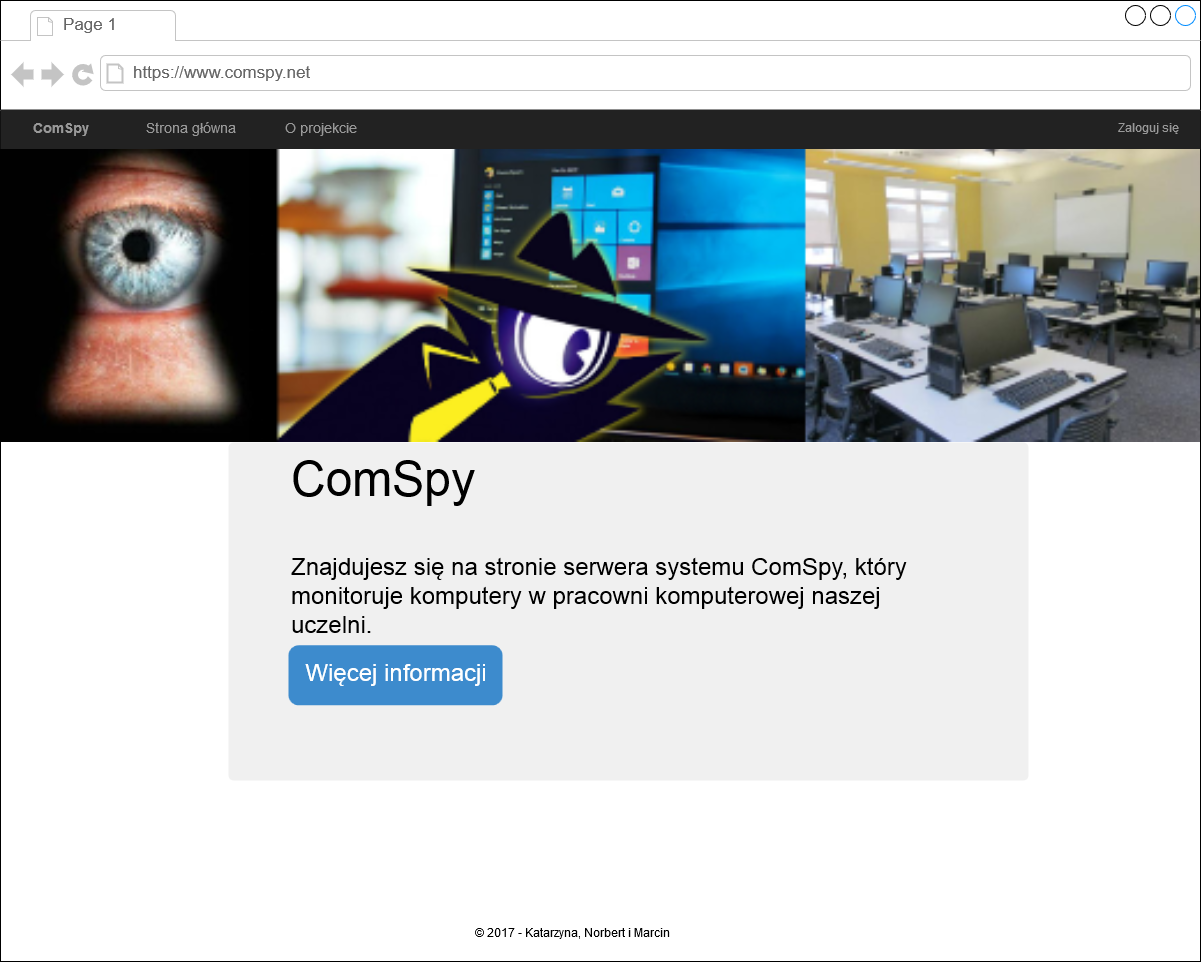
\includegraphics[height=12cm,width=15cm]{interfejs_homepage}
    \caption{Projekt strony głównej}
    \label{fig:my_label}
\end{figure}

\newpage
Rysunek nr 9 przedstawia panel logowania. W celu zalogowania się użytkownik jest proszony o podanie loginu i hasła. W przypadku wprowadzenia złych danych jest wyświetlany komunikat o błędzie i niepowodzeniu logowania.
\begin{figure} [!ht]
    \centering
    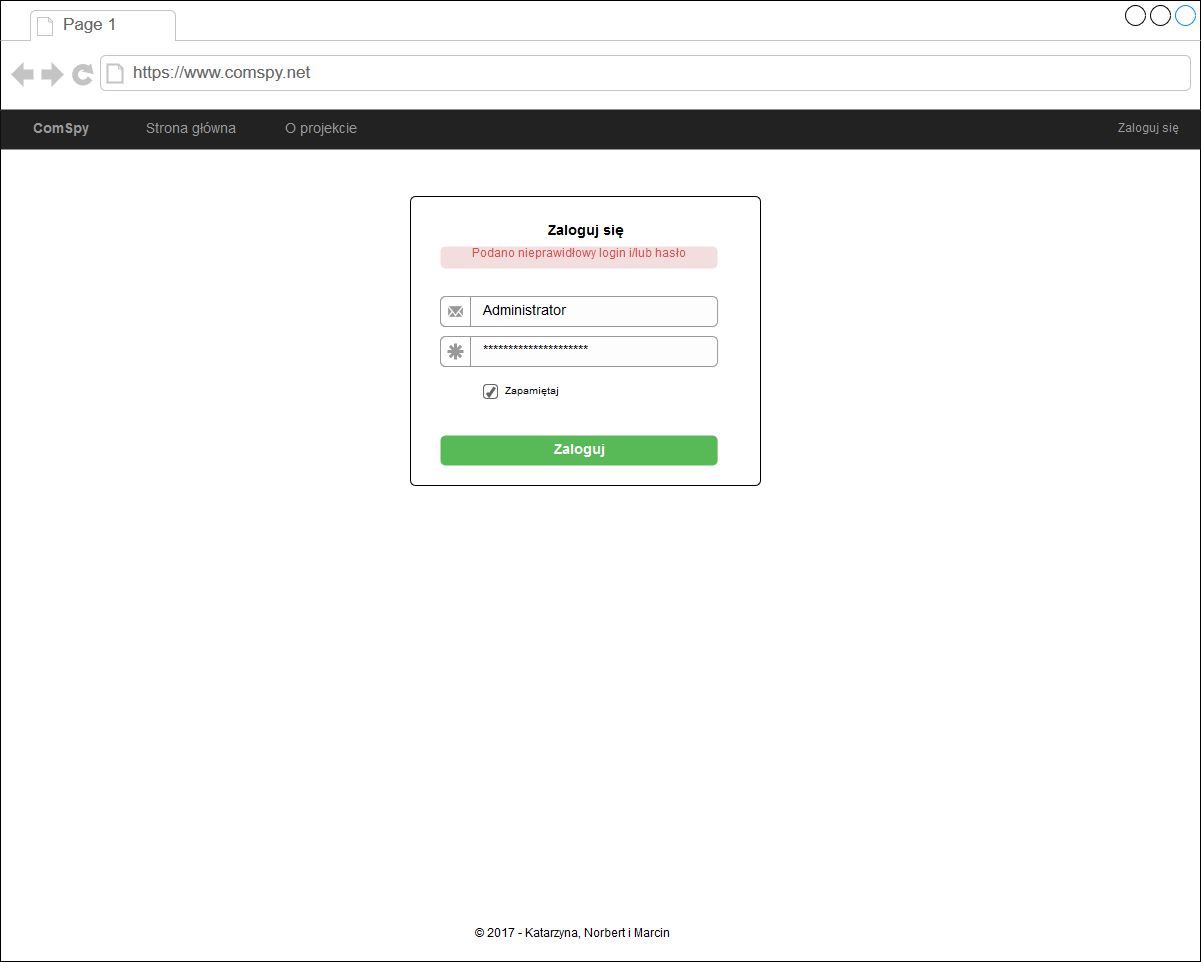
\includegraphics[height=12cm,width=15cm]{interfejs_zaloguj}
    \caption{Projekt strony logowania}
    \label{fig:my_label}
\end{figure}

\newpage
Rysunek nr 10 przedstawia projekt strony poglądu głównego, który jest widoczny dla użytkowników zalogowanych (oraz Administratorów). Widać tutaj podglądy wybranych przez użytkownika grup stanowisk oraz okienka z ostrzeżeniami związanymi z naruszeniem listy dozwolonych stron do przeglądania (blacklist)
\begin{figure} [!ht]
    \centering
    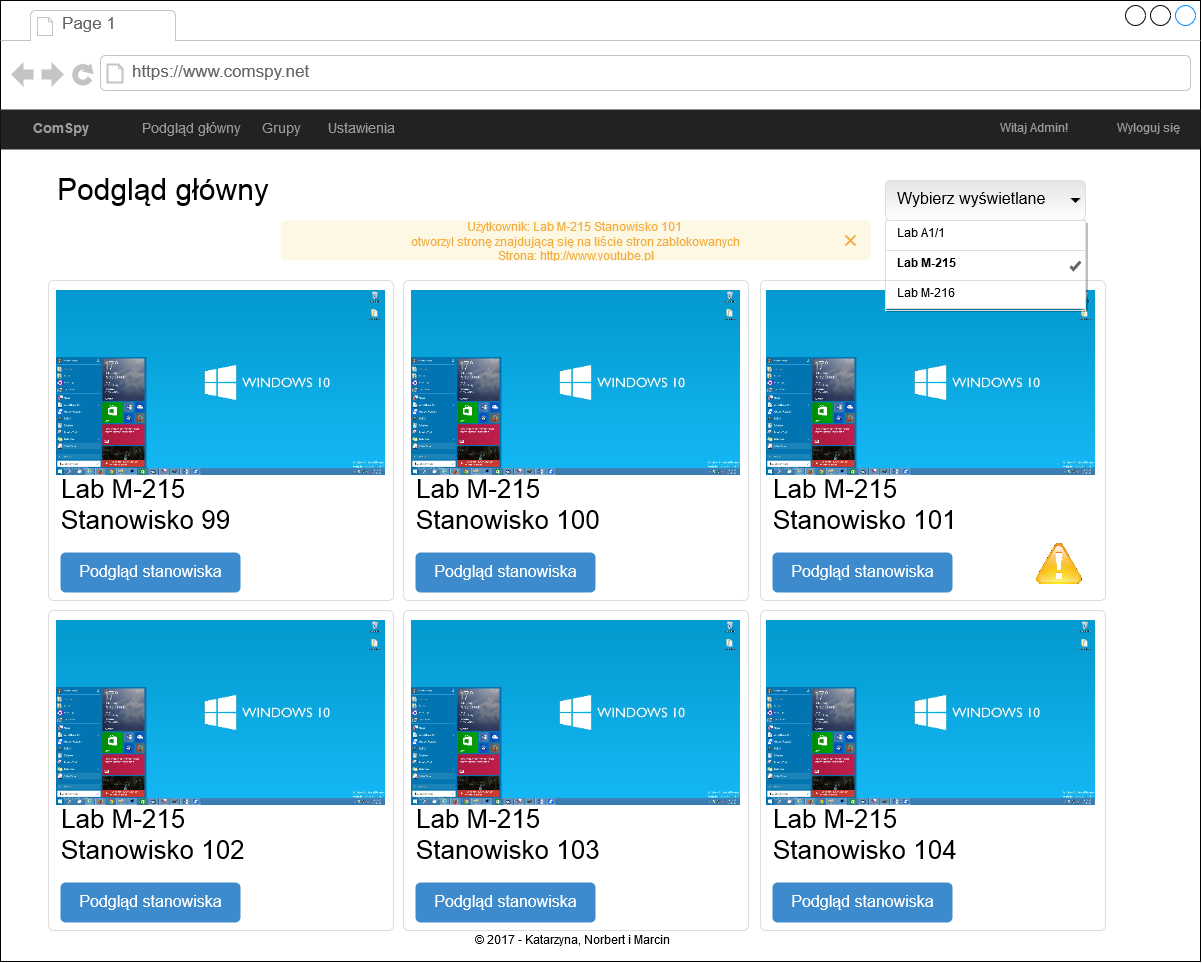
\includegraphics[height=12cm,width=15cm]{interfejs_podglad_glowny}
    \caption{Projekt strony - podgląd główny (dostępny po zalogowaniu)}
    \label{fig:my_label}
\end{figure}


\newpage
Rysunek nr 11 przedstawia projekt podglądu szczegółowego jednego stanowiska. Tutaj oprócz samego zrzutu ekranu wyświetlane są informacje o uruchomionych procesach, otwartych stronach internetowych oraz podstawowe dane konfiguracyjne.
\begin{figure} [!ht]
    \centering
    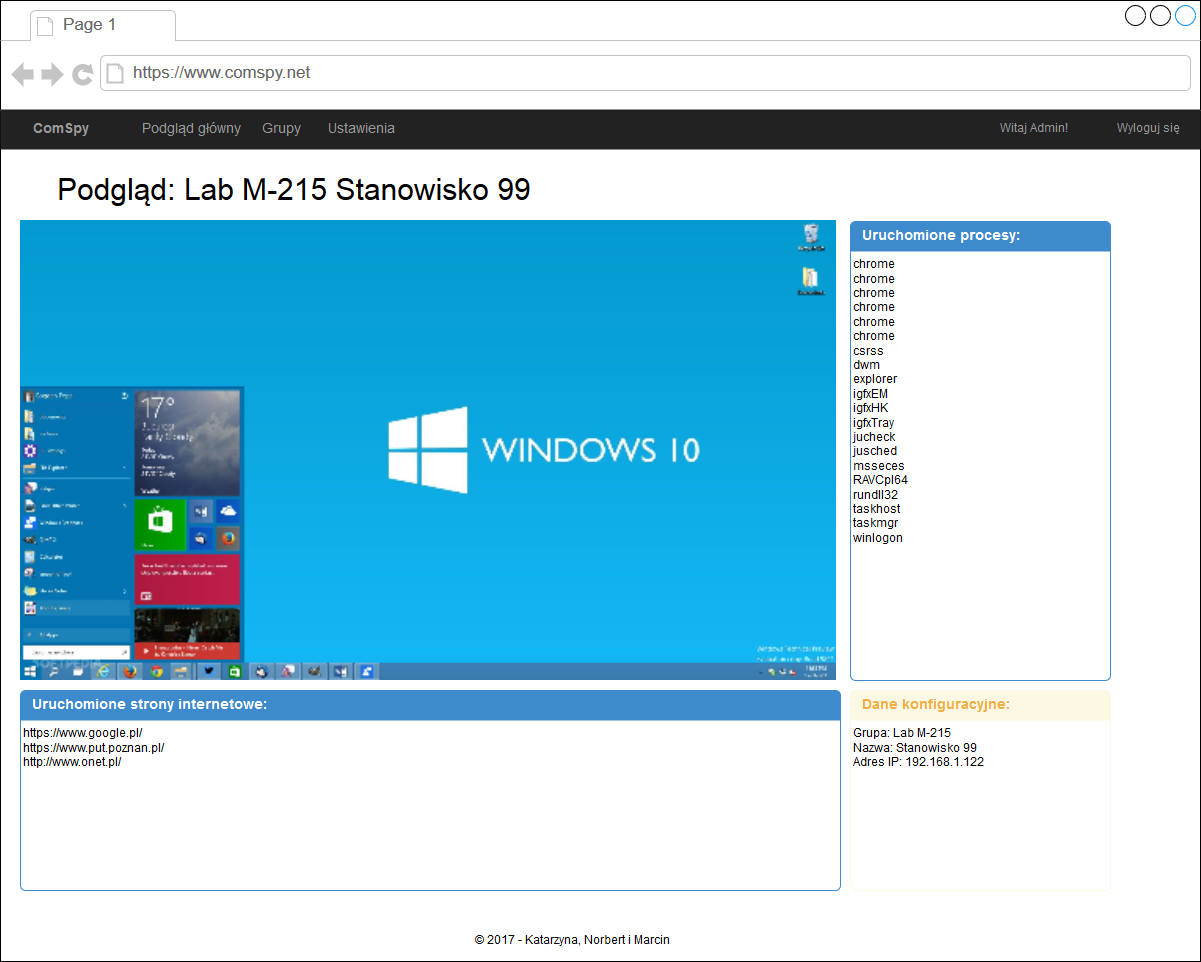
\includegraphics[height=12cm,width=15cm]{interfejs_podglad_stanowiska}
    \caption{Projekt strony - podgląd stanowiska (dostępny po zalogowaniu)}
    \label{fig:my_label}
\end{figure}


\newpage
Rysunek nr 12 przedstawia zarządzanie grupami oraz stanowiskami w ramach jednej z nich. Ten widok dostępny jest tylko dla administratorów.
\begin{figure} [!ht]
    \centering
    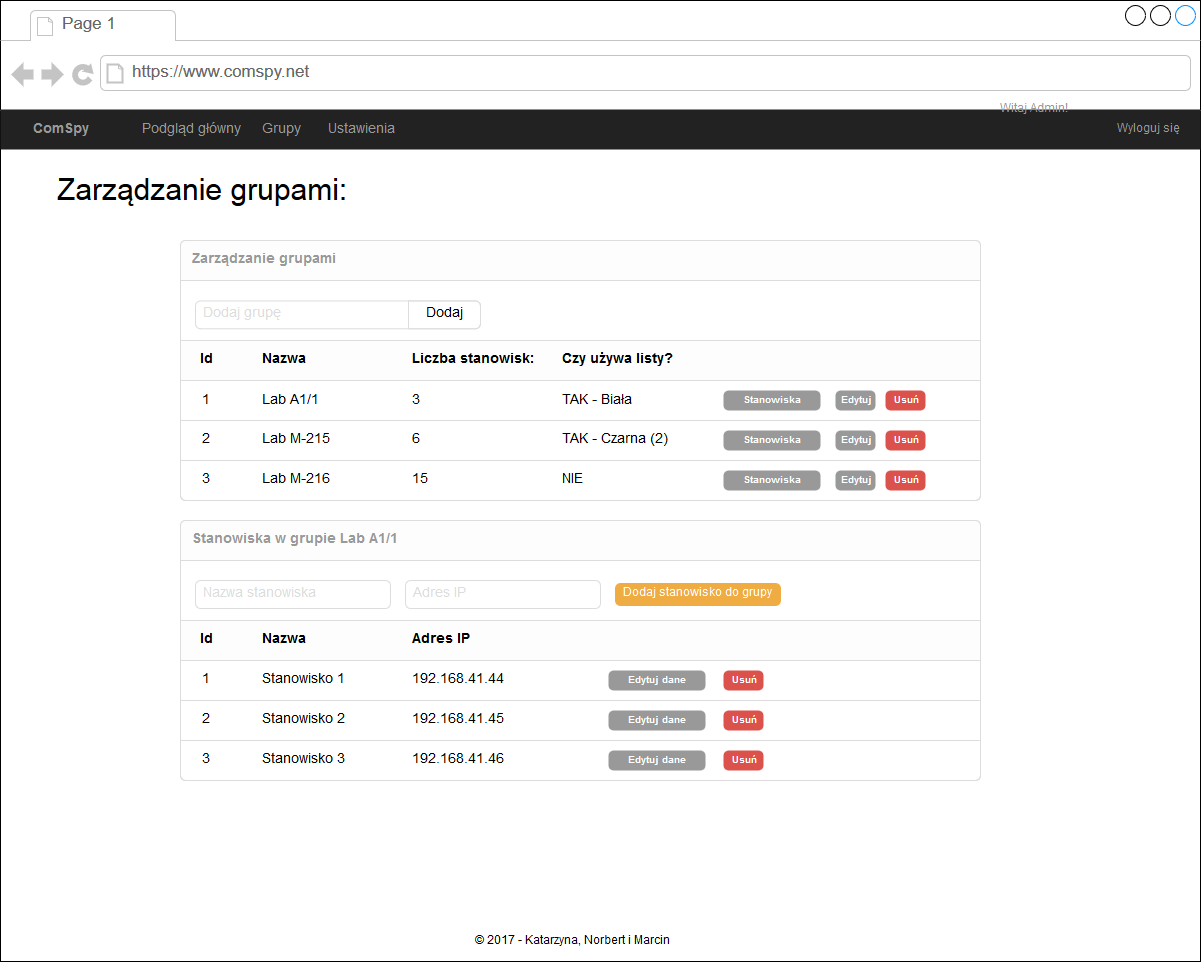
\includegraphics[height=12cm,width=15cm]{interfejs_grupy}
    \caption{Projekt strony - zarządzanie grupami i stanowiskami (dostępny po zalogowaniu)}
    \label{fig:my_label}
\end{figure}


\newpage
Rysunek nr 13 przestawia panele dotyczące zarządzania użytkownikami oraz blacklistą.
\begin{figure} [!ht]
    \centering
    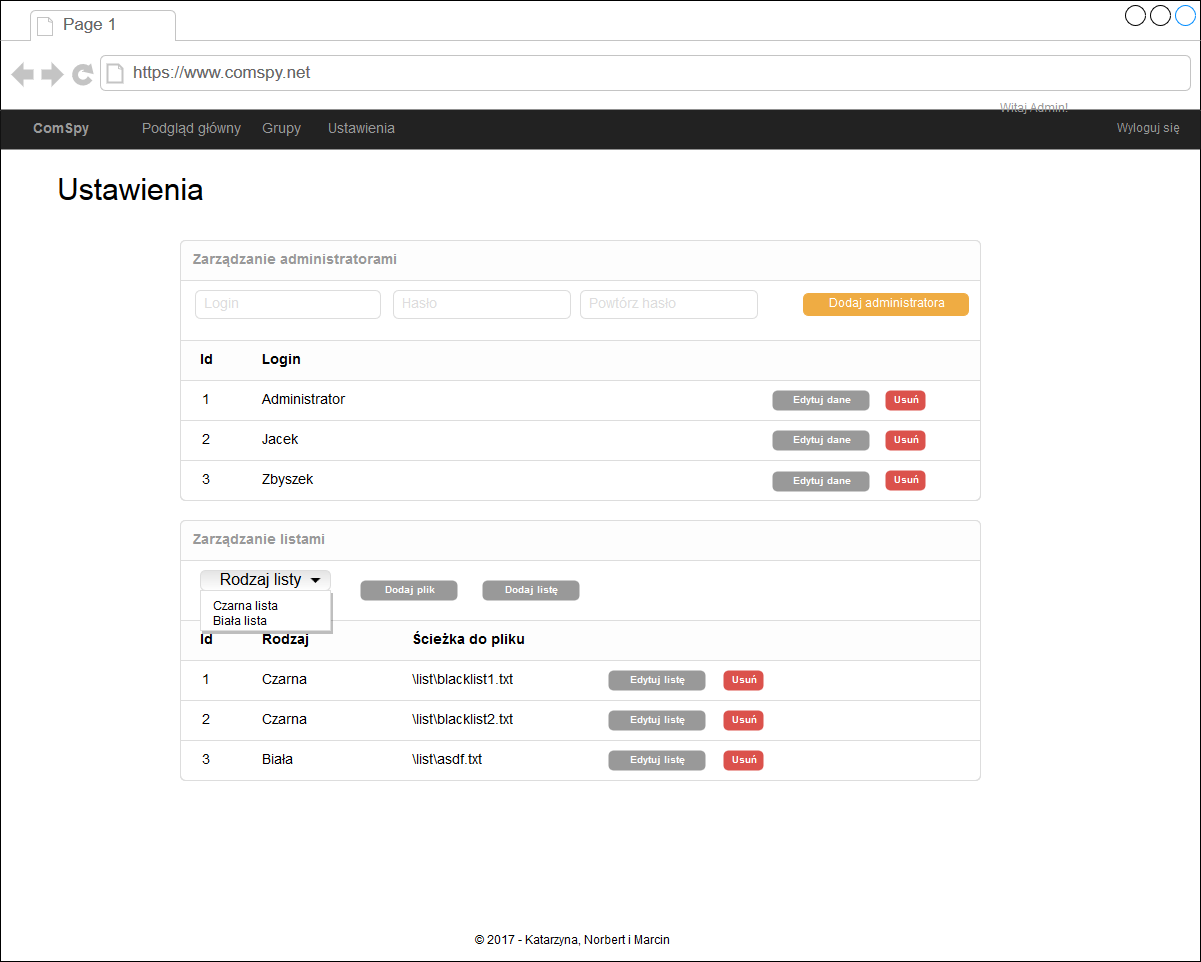
\includegraphics[height=12cm,width=15cm]{interfejs_ustawienia}
    \caption{Projekt strony - ustawienia (dostępny po zalogowaniu)}
    \label{fig:my_label}
\end{figure}


\newpage

\subsection{Aplikacja kliencka}
Ostatni szkic przedstawia program klienta, na którym widać niepodłączonego jeszcze klienta do serwera. Oprócz samego statusu połączenia widać adres IP serwera oraz identyfikator stanowiska. Widać także przyciski Podgląd, która przeniesie do okna, w którym można podejrzeć chwilowy stan tego, co jest następnie przesyłane do serwera. Po kliknięciu w przycisk Administrator natomiast można natomiast w przyszłości zaimplementować podstawowy panel administracyjny lub inne funkcje, które dostępne będą tylko dla administratora systemu.


\begin{figure} [!ht]
    \centering
    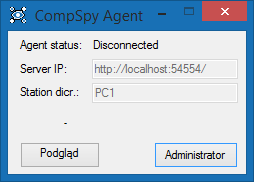
\includegraphics[height=6cm,width=8cm]{interfejs_agent}
    \caption{Projekt strony - ustawienia (dostępny po zalogowaniu)}
    \label{fig:my_label}
\end{figure}